\maketitle

인생은 한 번뿐이니 당장 내가 원하는 것을 하겠다는 `욜로(YOLO, You Only Live Once)' 열풍이 언제 불었냐는 듯, 코로나가 한국 사회를 강타한 2020년 이후로는 `갓생' 키워드가 광범위하게 언급되기 시작했다. `갓생'은 신을 의미하는 영어 단어 `갓(god)'과 인생을 가리키는 `생(生)'을 합친 합성어다. 구체적으로 무엇이 `갓생'인가에 대한 엄밀한 정의는 없지만, 대체로 꾸준한 공부와 운동 등 자기관리를 통해 생산적이고 계획적인 삶을 뜻하는 것으로 통용된다. `갓생'은 완성된 형태의 삶을 의미하는 것 이상으로, 그런 삶을 이룩하기 위한 자기계발의 과정까지 포괄한다. 유튜브나 인스타그램과 같은 소셜미디어에서 ``갓생" 키워드를 검색해보면 빼곡한 노트 필기와 스케줄 표, 운동 기록, 바디 프로필\footnote{운동과 식단관리로 매력적인 신체를 만든 뒤 스튜디오에서 촬영한 사진.} 콘텐츠가 화면을 가득 채우는 것을 볼 수 있다.

나는 `갓생' 트렌드가 본질적으로 자기계발 담론과 다르지 않다는 문제의식을 바탕으로, `갓생'과 같은 자기계발 담론이 신자유주의 이데올로기를 지지, 강화한다는 해석을 제시하고자 한다. 대부분의 미디어는 `갓생' 트렌드를 MZ세대(1980년대 초반부터 2010년대 후반에 출생한 세대)가 자아 성취를 달성하는 새로운 방식으로 긍정 평가하고 있다. `갓생' 트렌드는 자기계발과 달리 외면이 아닌 내면의 성장에 초점이 맞춰져 있다는 것이다. 그러나 실제로는 `갓생' 트렌드도 기존의 자기계발 담론과 다를 바 없이 개인의 의지와 노력을 강조한다는 점, 그리고 그 기저에는 미래에 대한 불안의 조건과 감정이 깔려 있다는 점\cite{csy2022}에서 비판적으로 고찰해볼 필요가 있다. 이 글에서는 '갓생' 트렌드를 비롯한 자기계발 담론이 어떤 신자유주의 이데올로기를 담아내는지 논한 다음, 미디어가 어떻게 이를 재현하는지 살펴보고자 한다.

\section*{자기계발 담론의 신자유주의 이데올로기}

자기계발 담론으로서의 `갓생' 트렌드를 주도하는 Z세대(1990년대 초반부터 2010년대 후반에 출생한 세대)는 신자유주의가 한국에 이식된 1990년대 후반에 청소년기를 보냈거나, 그 이후에 출생했다는 점에서 이 새로운 자기계발 담론을 주의 깊게 살펴봐야 한다. Z세대가 단순히 개인주의적이라는 편견적 인식을 넘어, 본격적인 신자유주의 사회 구조 안에서 자란 세대 집단에게 자기계발 담론은 불가피한 생존전략으로 작용했을 가능성이 충분하기 때문이다.

자기계발 담론은 1997년 외환위기 이후 한국에 신자유주의 질서가 자리잡은 뒤로 2000년대 내내 전성기를 누렸다. 신자유주의 기조 아래 정부와 법인세, 규제, 복지는 자유시장과 세계화의 적으로 간주되었으며, 이 시기 대폭 축소된 사회 안전망의 사각지대에서 개개인은 파편화되어 각자도생해야 했다. 신자유주의는 경제학적 사조를 넘어 이데올로기로서 작동했다. 신자유주의 이데올로기는 경쟁 사회에서 도태되지 않으려면 개인이 스스로를 갈고 닦아 승리를 쟁취해야 하며, 실제로도 그것이 가능하다는 성공 신화를 지어냈다. 이러한 성공 신화를 기반으로 번성한 전통적 자기계발 담론은 2008년 서브프라임 모기지 사태로 금융위기가 일어나며 주춤했다. 2010년대는 자기계발 담론의 연장선상에서 힐링 담론이 주류를 차지하며 심리적 자기계발로 흐름이 전환된다\cite{lws2018}. 또 한편으로는 `헬조선'과 같은 냉소주의나 `욜로'와 같은 허무주의가 청년 세대의 트렌드를 주도하기도 했다. 그러다가 2020년 코로나로 인해 불확실성이 커지고, 성장의 가능성이 줄어들면서 전통적 자기계발 담론은 생산적이고 계획적인 삶을 사는 `갓생'이라는 화려한 겉모습으로 복귀했다. 급격한 인플레이션과 전 세계적인 우경화, 기후 위기의 체감, 인구 절벽, 개인을 무력하게 만드는 거대한 시대적 흐름을 당면한 한국의 2022년 하반기는 자기계발 담론이 꽃 피우기에 최적의 환경을 조성하고 있다.

`갓생'을 사는 데 필요한 자원은 돈과 시간, 건강 등으로 정형화되어 있는 반면, `갓생'을 사는 것이 불가능한 원인은 다양하다. 하지만 `갓생'을 향한 찬양은 너무나도 쉽게 그렇지 않은 삶에 대한 비난으로 이어지곤 한다. 자기계발 담론은 개인을 둘러싼 사회 구조적 맥락을 은폐하여 인식의 틀을 납작하게 만들고, 결국 개인의 노력만을 강조한다는 점에서 구조맹(構造盲)을 양산하는 결과를 초래한다. 당장 닥친 문제에 대해 구조적 원인과 해결책을 고민하는 것보다는, 모든 것을 개인의 문제로 환원하는 것이 더욱 직접적이고 확실한 해결책인 듯 인식하는 것이다. 자기계발 담론은 신자유주의 이데올로기를 재생산하며 사회 이동에 개인의 역량이 대단히 큰 영향을 미치고, 누구나 노력만 하면 사회적으로 성공할 수 있다는 성공 신화를 설파한다. 성공 신화를 신봉하는 사회에서 노력하지 않는 개인은 사회에 기여하지 않고 혜택만을 취하는 무임승차자\cite{och2013}로 취급된다. 무임승차자는 도덕적 비난을 받아야 함이 마땅하며, 그에 상당한 사회적 처벌까지도 받아야 한다. `인서울' 대학교에 진학하지 못한 것은 학창 시절의 게으름에 대한 공정한 처벌이다. 정규직으로 취업하지 못한 것은 스펙을 쌓지 않은 게으름에 대한 공정한 처벌이다. 궁극적으로 가난은 개인이 삶 전반에서 누적해온 게으름에 대한 종합 처벌인 셈이다.

그러나 현대 사회에서 개인은 끊임없이 환경의 영향을 받으며, 의지와 노력만으로는 자신의 상황을 통제할 수 없게 만드는 거대한 구조 앞에 무력해진다. 부의 대물림과 계급 세습이 사회 문제로 부각된 것은 이미 오래전이다. 가난한 개인들은 줄어들어 가는 일자리를 놓고 서로를 밟고 올라서야 하는 경쟁의 구조 안에 속박되어 있다. 그럼에도 자기계발 담론은 끊임없이 개인의 계급 상승을 추동한다. 피지배계급은 자신의 계급 문제에서 소외되어 언젠가는 노력을 통해 부를 쌓고 지배계급이 될 `부자 준비생'으로 정체화된다. 이렇게 개인은 불평등을 자연스러운 것으로 받아들이고, 계급 피라미드 안에서 최정상에 서는 것만이 자신에게 주어진 성공의 길이라는 신자유주의 이데올로기를 내면화한다. Z세대의 새로운 자기계발 담론은 더 이상 게임의 규칙을 바꿀 수 없게 된 좌절의 현장에서, 차라리 최대한 규칙에 충실하여 게임의 승리자로 올라서고자 하는 분투에 가깝다.

\section*{미디어가 제시하는 `갓생'의 과정과 목표}

Z세대를 타겟팅하는 방송도 `갓생' 트렌드를 놓치지 않았다. tvN <유 퀴즈 온 더 블럭> 86화에는 `미라클모닝'을 실천하는 변호사가 출연했다. `미라클모닝'은 미국의 성공 코치 할 엘로드(Hal Elrod)가 2016년 자신의 저서 <미라클모닝>에서 소개한 자기 관리 습관으로, 매일 새벽 4시 30분에 기상하여 자기계발 활동을 하는 것이 핵심이다. <유 퀴즈 온 더 블럭>에서 ``존경하는 분들이 오전 6시에 모여 조찬을 즐기는 모습을 보고 `미라클모닝'을 결심했다"는 변호사의 자기계발 서사는 `미라클모닝'이 2000년대 초 유행했던 `아침형인간'과 그대로 맞닿아있음을 단적으로 보여준다. 변호사가 자신이 존경하던 이들처럼 되기 위해 `미라클모닝'을 결심했듯이, 방송을 통해 변호사를 본 수용자도 `미라클모닝'을 결심하며 사회적으로 인정받는 커리어를 달성할 수 있다는 자기계발 성공 신화가 재생산된다.

미디어는 완성된 형태인 결과로서의 `갓생'을 제시하며 자기계발 차원에서 과정으로서의 `갓생'이 추구해야 할 목표 가치를 설정한다. 미디어에 노출되는 결과로서의 `갓생' 이미지는 주로 사회초년생이나 대학생이 해외여행이나 오마카세, 명품 등 거금이 드는 소비를 `플렉스'하는 모습이나, 신체적 건강함과 섹슈얼리티를 강조하는 바디 프로필의 모습으로 실현된다. 이렇게 보여지는 화려한 `갓생'의 상징은 그 이면에 있는 계급과 불평등, 신체적 정상성에 대한 입체적 문제의식을 희석하고, 결국 `나도 저렇게 되고 싶다'라는 선망의 대상으로 거듭난다.

그런 측면에서 미디어가 뷰티 유튜버 `프리지아'를 통해 재현한 `갓생'의 이미지도 짚고 넘어갈 만하다. 미디어에 그려진 `프리지아'는 성수동 고층 아파트에 거주하며 고가의 명품을 착용하고 취미로 유화와 골프를 즐기는 대학생으로, 누구나 선망할만한 `갓생'을 살아간다. 넷플릭스 <솔로지옥> 출연 후 급격히 대중의 관심을 받은 `프리지아'는 얼마 지나지 않아 거주하고 있는 집이 자가가 아닌 월세였다는 논란과, 착용한 명품이 가품이었다는 논란에 휩싸였다. 그런데 `프리지아'를 둘러싼 논란은 대중을 기만한 것에 대한 배신감 또는 상류층의 자격을 재평가하는 수준이었고, 사치스러운 젊은 여성이라는 여성혐오적 맥락으로 이어지는 그릇된 양상까지 보이기도 했다. 그전에 미디어가 계급 세습과 불평등을 선망의 대상으로 그려내는 방식은 전혀 비판의 대상이 되지 않았다.

MBC <공유의 집> 1화에서는 ``초고층 럭셔리 준수의 소유하우스''라는 제목을 걸고 가수 `김준수'의 집을 소개했다. 스튜디오의 패널들은 넓은 실내 공간과 고급스러운 인테리어, 명품으로 가득 찬 드레스룸을 보며 연신 감탄을 내뱉는다.
\begin{figure}[h]
  \centering
  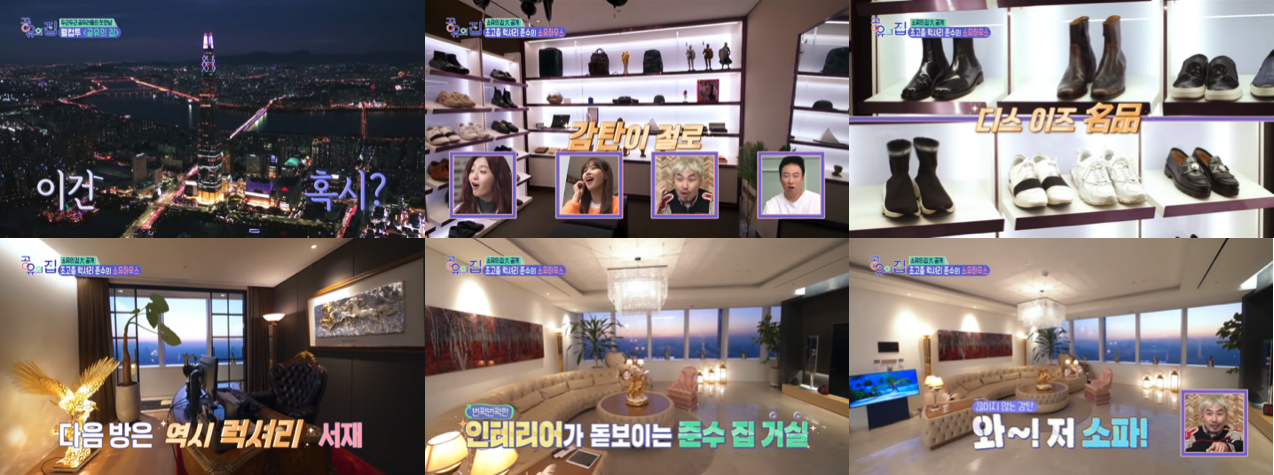
\includegraphics[width=\textwidth]{mbc2019.png}
  \caption{MBC <공유의 집> 1화 ``초고층 럭셔리 준수의 소유하우스''}
  \label{fig:mbc2019}
\end{figure}
롤랑 바르트(Roland Gérard Barthes)는 언어학적 체계로서의 1차 의미작용을 확장해 신화적 체계로서의 2차 의미작용을 정의했다. 바르트에 따르면 1차 의미작용의 기표, 기의, 기호는 2차 의미작용을 통해 또 다른 의미를 파생시킨다. <공유의 집> 1화에서 처음 집을 소개하는 장면을 \cnm{그림 \ref{fig:barthes-table}}와 같이 바르트의 2단계 의미작용 모형으로 표현해보면 방송이 노골적으로 상류층에 대한 선망의 기호을 재생산했음을 알 수 있다.
\begin{figure}[h]
  \centering
  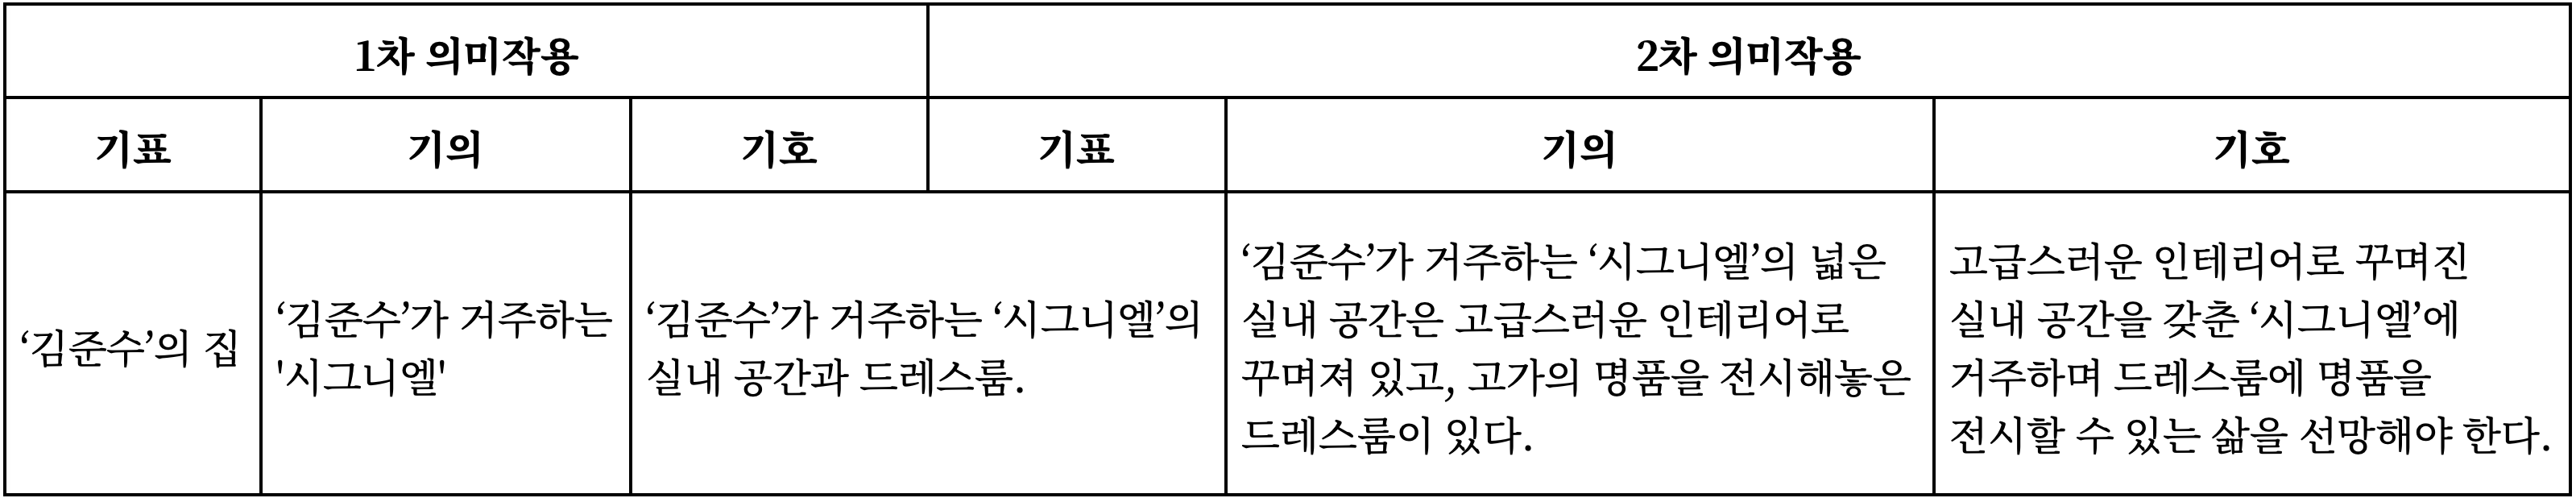
\includegraphics[width=\textwidth]{barthes-table.png}
  \caption{MBC <공유의 집> 1화에 대한 바르트 2단계 의미작용 분석}
  \label{fig:barthes-table}
\end{figure}
\cnm{그림 \ref{fig:mbc2019}}의 장면에서 1차 의미작용의 기호는 단순히 ``가수 `김준수'가 거주하는 `시그니엘'\footnote{서울 송파구의 롯데월드타워에 위치한 고급 오피스텔.}''이지만, 2차 의미작용의 기호는 ``고급스러운 인테리어로 꾸며진 실내 공간을 갖춘 `시그니엘'에 거주하며 드레스룸에 명품을 전시할 수 있는 삶을 선망해야 한다.''라는 상류층 선망 신화로 이어진다. 미디어가 상류층을 향한 일방적인 선망의 기호를 재생산하는 것이 위험한 이유는, 이러한 기호가 수용자로 하여금 계급 배반적 가치관을 내면화하도록 만들며, 노동자가 노동자를 혐오하게 만들고, 최종적으로는 계급적 연대를 사전에 원천 봉쇄하기 때문이다.

`갓생' 트렌드가 이전의 자기계발 트렌드와 다른 점은 `갓생'의 이미지가 소셜미디어를 통해 개인의 단위에서 활발하게 재현된다는 점이다. 과정으로서의 `갓생'은 단순히 자기계발 활동을 통해 자기효능감을 얻는 것에서 그치지 않고, 소셜미디어에 이를 전시함으로써 완성된다. 유튜브, 인스타그램과 같은 소셜미디어에서 ``갓생" 키워드를 검색하면 \cnm{그림 \ref{fig:social-media}}과 같이 Z세대가 `갓생'을 인증하는 빼곡한 노트 필기, 스케줄표, 운동 기록, 바디 프로필 등의 콘텐츠를 쉽게 찾아볼 수 있다.
\begin{figure}[h]
  \centering
  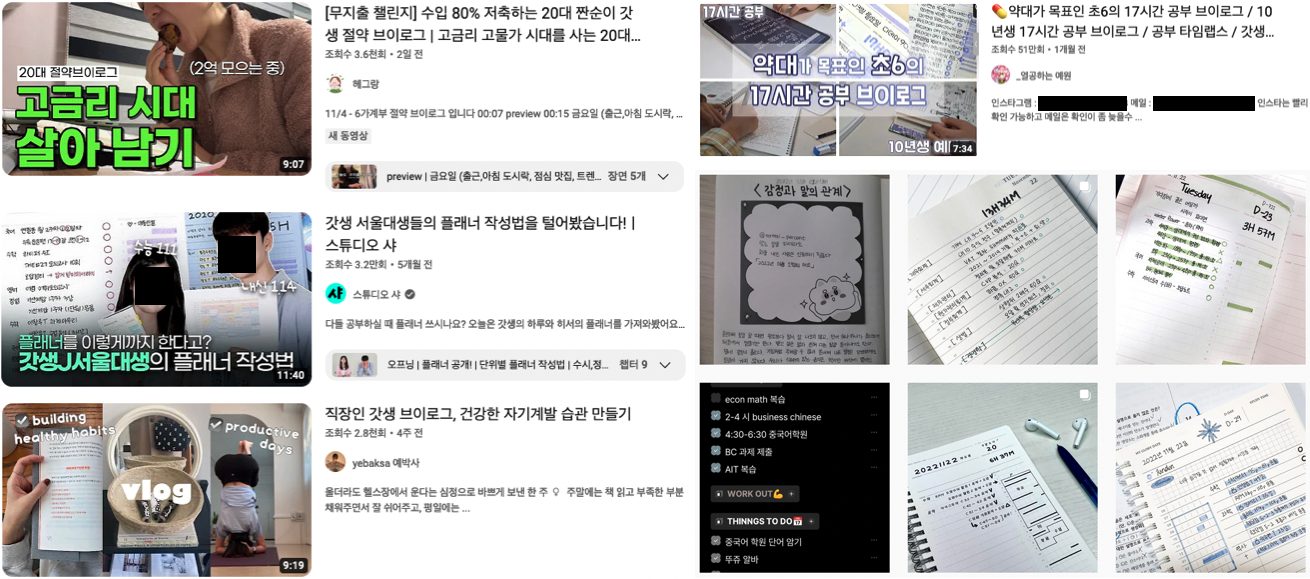
\includegraphics[width=\textwidth]{social-media.png}
  \caption{소셜미디어에서 재현되는 `갓생'의 이미지}
  \label{fig:social-media}
\end{figure}
\cite{ksh2022}은 아마추어 유튜버가 브이로그(Vlog)\footnote{개인적인 일상이나 경험, 생활을 촬영해 인터넷에 공개한 동영상.} 영상을 구성하기 위한 행위로 자기계발 활동을 선택하는 경향이 있으며, 구직 불안이 큰 20대에게는 이러한 브이로그 채널을 운영하는 것 자체가 하나의 스펙이 된다고 분석한다. 화려한 `갓생'의 밑바탕에 청년 세대의 불안이 있다는 것이다. 결국 소셜미디어에서는 타인의 자기계발 활동을 보며 불안을 느끼고, 불안해서 자기계발 활동을 하는 불안의 상호작용이 순환한다. 이 과정에서 형성된 자기계발 담론은 소셜미디어 특유의 빠른 속도로 신자유주의 이데올로기를 재생산한다.

\section*{불안을 먹으며 자라는 자기계발 담론}

미디어가 묘사하는 MZ세대는 자기 삶을 주체적으로 결정하고 개인을 중시하는 진취적인 모습이다. `갓생'을 비롯한 청년 세대의 자기계발 트렌드 역시 MZ세대라는 필터를 거치며 긍정적이고 건강한 측면만 강조되어 왔다. 그러나 실제 청년 세대는 미래의 불확실성과 포화된 노동 시장, 세밀하게 서열화된 계급 피라미드 속에서 끊임없는 성취를 요구받고 있다. 청년 개인은 성공 신화가 설파하는 실낱같은 희망을 붙잡고 자기계발을 이어갈 수밖에 없다. 하지만 성공 신화가 그려내는 약속되지 않은 미래는 불안을 가중할 뿐이다.

앞서 `갓생' 트렌드를 전통적 자기계발 담론의 복귀로 정의하며 한국에서 자기계발 담론이 어떻게 변화했는지 그 배경을 되짚어봤다. 자기계발 담론은 개인을 둘러싼 사회 구조적 맥락을 은폐하고, 개인의 역량만을 강조한다. 결국 자기계발 담론은 개인적인 차원에서 노력만 하면 사회적으로 성공할 수 있다는 신자유주의 이데올로기의 성공 신화를 낳는다. 이어서 미디어가 생산하는 `갓생'의 이미지를 두 가지 측면에서 분석했다. 과정으로서의 `갓생'은 자기계발 담론 아래에서 성공 신화를 재현한다. 미디어는 이미 사회적으로 성공을 인정받는 사람이 수행하는 자기계발 활동을 소개하며 성공 서사의 선후 관계를 왜곡한다. 또 다른 측면인 결과로서의 `갓생'은 상류층에 대한 선망의 이미지로 구체화된다. 미디어는 상류층의 소비와 화려한 일상을 연출하며 과정으로서의 `갓생'이 추구해야 할 신자유주의적 목표 가치를 제시한다. 마지막으로 두 측면의 `갓생' 이미지가 소셜미디어를 통해 개인의 단위에서도 활발하게 재현되고 있음을 언급했다. 그 동력은 청년 세대의 불안이며, 이 과정에서 빠르게 신자유주의 이데올로기가 재생산되고 있다.

만인이 만인의 경쟁자가 되어버린 각자도생의 사회에서 개인이 의지할 곳은 자신의 역량밖에 남지 않는다. 각자도생의 사회를 구축해낸 주역에는 미디어도 빠지지 않는다. 그런 미디어가 이제는 청년 세대의 자기계발을 장려하고 있다. 지금은 청년 세대가 자기계발밖에 할 수 없게 된 현실과 환경, 제도, 사회적 구조에 대한 본질적인 문제 제기가 필요한 시점으로 보인다.

\begin{thebibliography}{9}
  \bibitem[김소형, 2022]{ksh2022} 김소형, \snm{아마추어 브이로그 유튜버의 자기 계발 현상과 노동에 관한 연구}, \bnm{한국언론정보학보} 114호, 한국언론정보학회, 2022, 15쪽.
  \bibitem[최수이 $\cdot$ 김수정, 2022]{csy2022} 최수이 $\cdot$ 김수정, \snm{대학 청년의 MBTI 활용 담화에 나타난 앎의 의지와 지식-권력 효과}, \bnm{한국언론정보학보} 115호, 한국언론정보학회, 2022, 171쪽.
  \bibitem[오찬호, 2013]{och2013} 오찬호, ``우리는 차별에 찬성합니다", 개마고원, 2013.
  \bibitem[이원석, 2018]{lws2018} 이원석, ``대한민국 자기계발 연대기", 필로소픽, 2018.
\end{thebibliography}

